

\chapter{Environment and Source Codes} \label{app:env}

\section{Environment}

All fine-tuning and evaluation experiments were conducted on a single NVIDIA A100 40 GB SXM4 GPU. The software environment is listed in Table~\ref{tab:env}.

\begin{table}[h!]
\centering
\caption{Training and evaluation environment}
\label{tab:env}
\begin{tabular}{ll}
\hline
\textbf{Component} & \textbf{Version / Specification} \\
\hline
GPU                        & NVIDIA A100 40 GB SXM4 \\
CUDA                       & 12.1 \\
Python                     & 3.11 \\
PyTorch                    & 2.2.0 \\
Transformers (HuggingFace) & 4.40.0 \\
PEFT                       & 0.10.0 \\
bitsandbytes               & 0.43.0 \\
Flash Attention            & 2.5.6 \\
Accelerate                 & 0.29.0 \\
\hline
\end{tabular}
\end{table}

Quantization for deployment feasibility testing used the \textit{bitsandbytes} library with 4-bit NF4 format and double quantization enabled. Inference was served via a \textit{FastAPI} server to measure end-to-end latency, including image preprocessing and model generation time.

\section{Source Codes}

The implementation covers five main components: (1) the seven-step image enhancement pipeline, (2) dataset loading and caption formatting, (3) LoRA/DoRA fine-tuning via HuggingFace PEFT, (4) metric evaluation using the \textit{pycocoevalcap} library for BLEU, ROUGE-L, CIDEr, METEOR, and SPICE, and (5) the FastAPI inference server with 4-bit NF4 quantization.

Fine-tuning used the \textit{SFTTrainer} from TRL with the following training arguments common to all configurations: 3 training epochs, 8-bit paged AdamW optimizer, learning rate $2 \times 10^{-4}$, cosine learning rate scheduler with 100 warmup steps, per-device batch size of 2 with 8 gradient accumulation steps (effective batch size 16), and Flash Attention 2. The vision encoder was frozen in all experiments. All modules apply the same custom system prompt during training: \textit{``You are a VLM attached to an underwater robot. Describe the scene. Be concise but thorough.''}


\chapter{Datasets} \label{app:datasets}

\section{Li et al.\ Underwater Image Captioning Dataset}

The primary training and evaluation dataset is the underwater image captioning dataset introduced by Li et al.~\cite{mainref}. It contains 3,176 high-resolution underwater images across ten scene categories, with fish (1,861 images), coral reefs (1,587 images), and divers (850 images) being the most frequent. Each image is annotated with five distinct human-written captions contributed by volunteers with marine domain expertise, yielding 15,880 captions in total. Captions describe object morphology, color, quantity, motion, and scene context, providing vocabulary and syntactic diversity for training. Images were resized to $224 \times 224$ pixels for all experiments.

\begin{table}[h!]
\centering
\caption{Li et al.\ dataset statistics}
\label{tab:dataset_stats}
\begin{tabular}{lr}
\hline
\textbf{Statistic} & \textbf{Value} \\
\hline
Total images         & 3,176 \\
Captions per image   & 5 \\
Total captions       & 15,880 \\
Scene categories     & 10 \\
Image resolution     & $224 \times 224$ (resized) \\
\hline
\end{tabular}
\end{table}

\section{UWBench Dataset} \label{app:uwbench}

UWBench~\cite{uwbench} is used as an extended evaluation benchmark to assess ATHENA under more visually challenging conditions. Figure~\ref{fig:uwbench_construction} reproduces the construction overview from Zhang et al.~\cite{uwbench}.

\begin{figure}[h!]
    \centering
    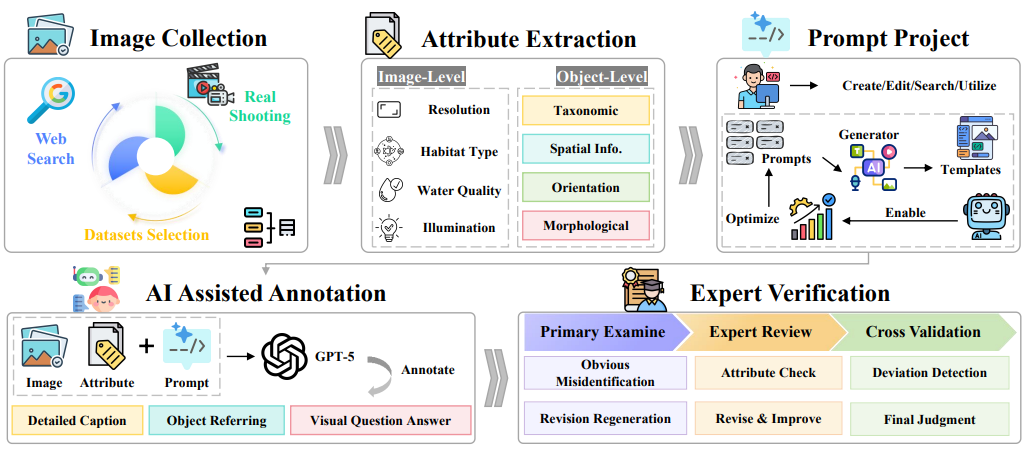
\includegraphics[width=\linewidth]{figures/uwbench_fig3.png}
    \caption{UWBench construction pipeline, reproduced from Zhang et al.~\cite{uwbench}.}
    \label{fig:uwbench_construction}
\end{figure}

\textbf{Image collection.} Images were gathered from web searches, existing underwater detection datasets, and in-situ robotic footage. From over 35,000 candidates, 15,003 were selected after filtering for quality, duplicates, and diversity across habitat type, water conditions, and scene complexity.

\textbf{Attribute extraction.} Each image was annotated with image-level attributes (habitat, water quality, illumination) and object-level attributes (taxonomy, bounding box, spatial relationships, morphology), which served as structured inputs to the annotation pipeline.

\textbf{AI-assisted annotation.} GPT-5 generated initial captions, object referring expressions, and visual QA pairs for each image using task-specific prompts grounded in the extracted attributes.

\textbf{Expert verification.} All outputs underwent three-stage review by marine biology experts: error checking by trained annotators, validation of taxonomic accuracy by senior biologists, and cross-validation of 2,000 images for inter-annotator agreement, totaling over 600 hours.

The resulting dataset contains 15,003 expert-verified captions, 15,281 object referring expressions, and 124,983 visual QA pairs. UWBench-Cap is partitioned into 10,454 training images and 4,549 test images.

\begin{table}[h!]
\centering
\caption{UWBench statistics}
\label{tab:uwbench_stats}
\begin{tabular}{lr}
\hline
\textbf{Statistic} & \textbf{Value} \\
\hline
Total images                 & 15,003 \\
Object categories            & 158 \\
Captions (avg.\ words)       & 68.6 \\
Object referring expressions & 15,281 \\
VQA pairs                    & 124,983 \\
Training split (Cap)         & 10,454 images \\
Test split (Cap)             & 4,549 images \\
\hline
\end{tabular}
\end{table}


\chapter{Full Experimental Results} \label{app:results}

\section{Backbone Hyperparameter Ablation}

Tables~\ref{tab:app_smolvlm} through~\ref{tab:app_qwen} report all 18 configurations from the backbone ablation on the Li et al.\ dataset. B-N, R-L, C, S, and M denote BLEU-N, ROUGE-L, CIDEr, SPICE, and METEOR; all metrics are on a 0--1 scale. Bold indicates the best result per metric within each backbone. Figure~\ref{fig:metrics_comparison} visualizes scores across all configurations simultaneously, grouped by backbone.

\begin{figure}[h!]
    \centering
    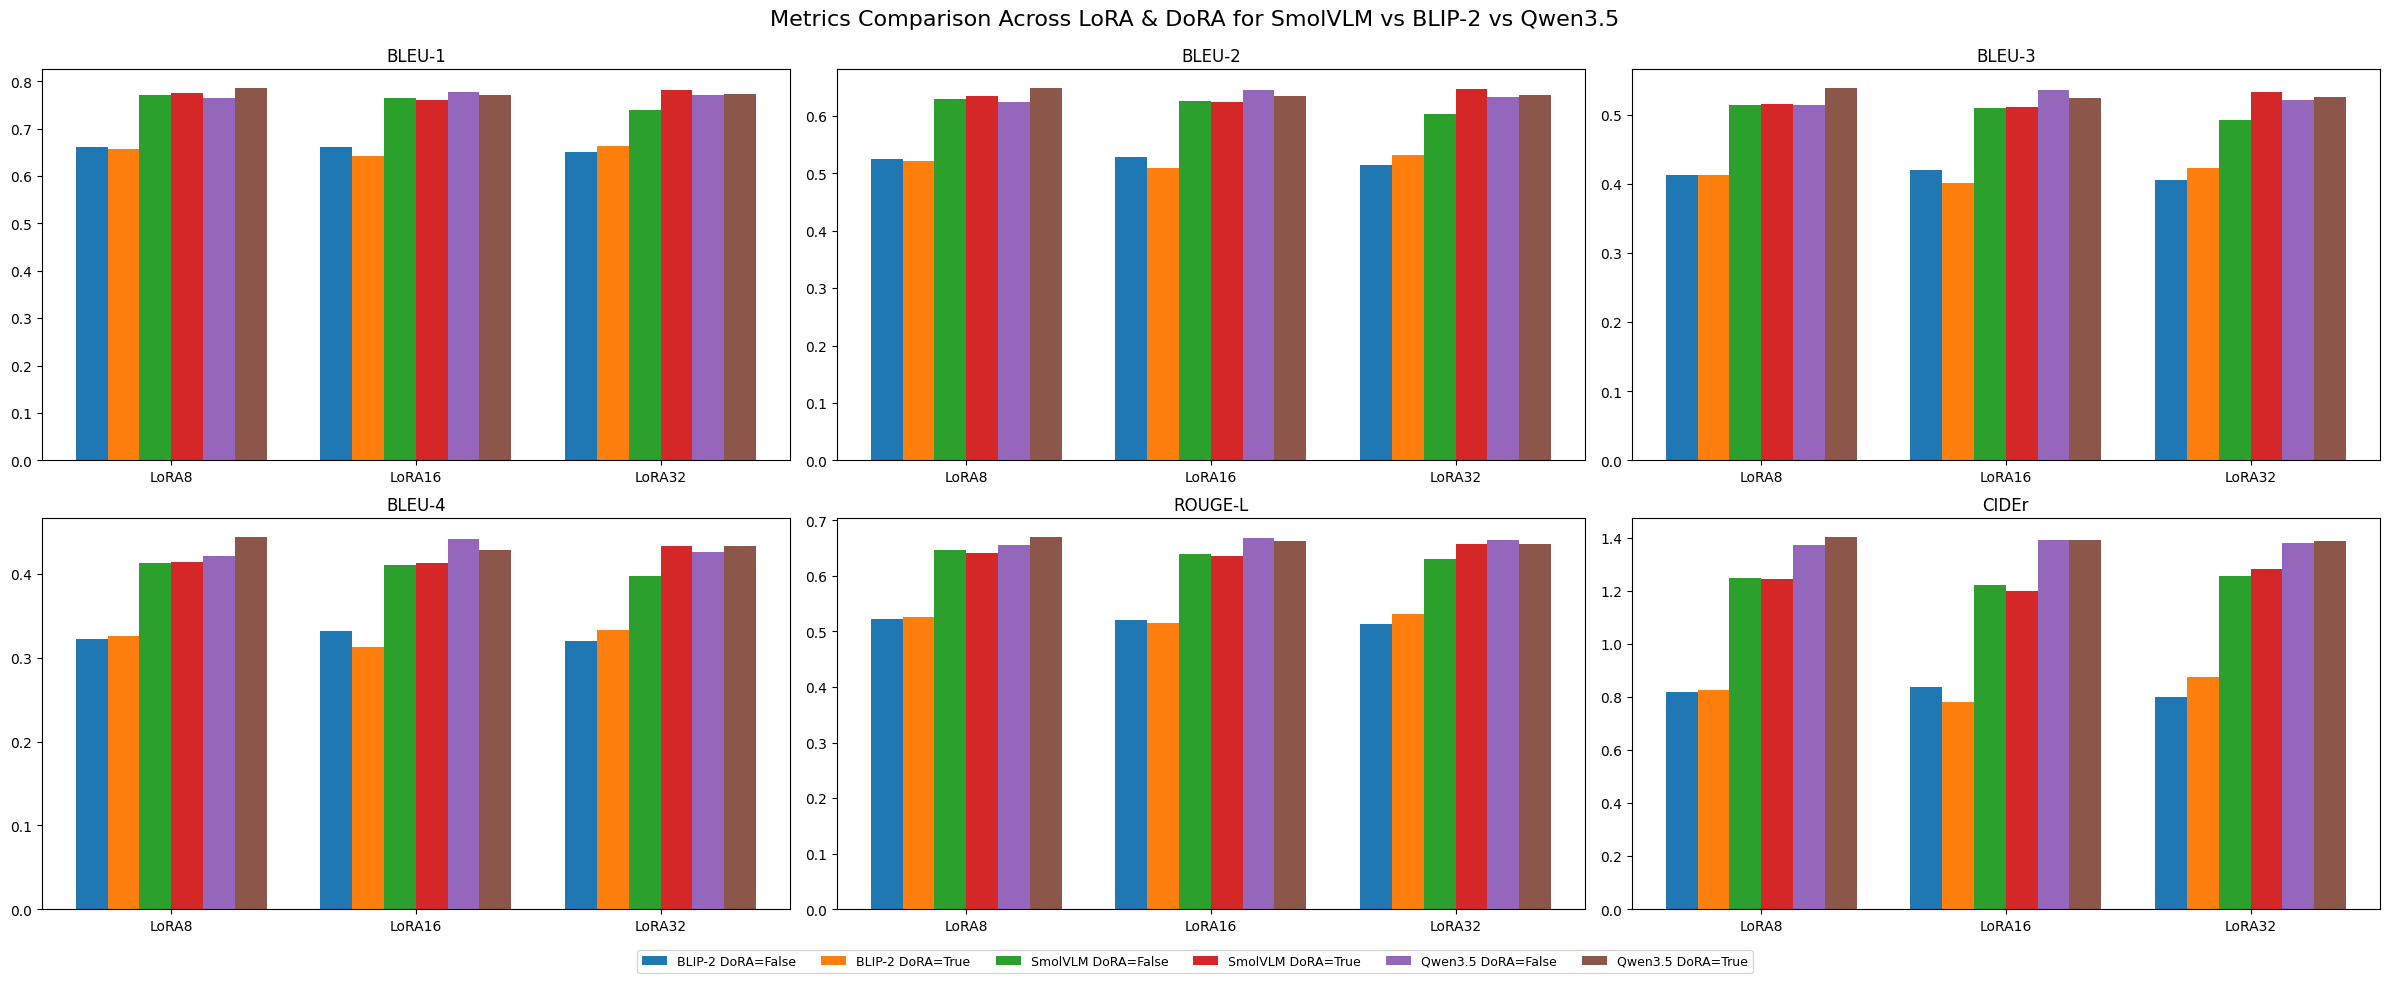
\includegraphics[width=\linewidth]{figures/metrics_comparison_hf.png}
    \caption{Metrics comparison across all 18 configurations, grouped by backbone.}
    \label{fig:metrics_comparison}
\end{figure}

\begin{table}[h!]
\centering
\caption{SmolVLM-Instruct: all configurations}
\label{tab:app_smolvlm}
\resizebox{\columnwidth}{!}{%
\begin{tabular}{llcccccccc}
\hline
\textbf{Model} & \textbf{Config} & \textbf{B-1} & \textbf{B-2} & \textbf{B-3} & \textbf{B-4} & \textbf{R-L} & \textbf{C} & \textbf{S} & \textbf{M} \\
\hline
SmolVLM & LoRA8  DoRA=N & 0.7710 & 0.6300 & 0.5169 & 0.4137 & 0.6466 & 1.2475 & 0.2675 & 0.3301 \\
SmolVLM & LoRA8  DoRA=Y & 0.7760 & 0.6339 & 0.5160 & 0.4148 & 0.6419 & 1.2449 & \textbf{0.2723} & \textbf{0.3325} \\
SmolVLM & LoRA16 DoRA=N & 0.7651 & 0.6256 & 0.5106 & 0.4103 & 0.6398 & 1.2234 & 0.2616 & 0.3247 \\
SmolVLM & LoRA16 DoRA=Y & 0.7611 & 0.6240 & 0.5116 & 0.4126 & 0.6358 & 1.1988 & 0.2639 & 0.3247 \\
SmolVLM & LoRA32 DoRA=N & 0.7398 & 0.6027 & 0.4931 & 0.3979 & 0.6307 & 1.2563 & 0.2569 & 0.3236 \\
SmolVLM & LoRA32 DoRA=Y & \textbf{0.7820} & \textbf{0.6474} & \textbf{0.5327} & \textbf{0.4332} & \textbf{0.6574} & \textbf{1.2810} & 0.2610 & 0.3241 \\
\hline
\end{tabular}%
}
\end{table}

\begin{table}[h!]
\centering
\caption{BLIP-2 OPT 2.7B: all configurations}
\label{tab:app_blip2}
\resizebox{\columnwidth}{!}{%
\begin{tabular}{llcccccccc}
\hline
\textbf{Model} & \textbf{Config} & \textbf{B-1} & \textbf{B-2} & \textbf{B-3} & \textbf{B-4} & \textbf{R-L} & \textbf{C} & \textbf{S} & \textbf{M} \\
\hline
BLIP-2 & LoRA8  DoRA=N & 0.6612 & 0.5247 & 0.4124 & 0.3220 & 0.5218 & 0.8209 & 0.2656 & 0.3230 \\
BLIP-2 & LoRA8  DoRA=Y & 0.6564 & 0.5217 & 0.4134 & 0.3257 & 0.5252 & 0.8206 & \textbf{0.2793} & 0.3328 \\
BLIP-2 & LoRA16 DoRA=N & 0.6610 & 0.5275 & 0.4198 & 0.3318 & 0.5209 & 0.8387 & 0.2698 & 0.3279 \\
BLIP-2 & LoRA16 DoRA=Y & 0.6434 & 0.5093 & 0.4009 & 0.3131 & 0.5146 & 0.7798 & 0.2608 & 0.3196 \\
BLIP-2 & LoRA32 DoRA=N & 0.6498 & 0.5142 & 0.4053 & 0.3198 & 0.5140 & 0.7996 & 0.2668 & 0.3232 \\
BLIP-2 & LoRA32 DoRA=Y & \textbf{0.6639} & \textbf{0.5317} & \textbf{0.4229} & \textbf{0.3335} & \textbf{0.5322} & \textbf{0.8740} & 0.2709 & \textbf{0.3335} \\
\hline
\end{tabular}%
}
\end{table}

\begin{table}[h!]
\centering
\caption{Qwen3.5-VL: all configurations}
\label{tab:app_qwen}
\resizebox{\columnwidth}{!}{%
\begin{tabular}{llcccccccc}
\hline
\textbf{Model} & \textbf{Config} & \textbf{B-1} & \textbf{B-2} & \textbf{B-3} & \textbf{B-4} & \textbf{R-L} & \textbf{C} & \textbf{S} & \textbf{M} \\
\hline
Qwen3.5 & LoRA8  DoRA=N & 0.7809 & 0.6467 & 0.5390 & 0.4474 & 0.6740 & 1.4234 & 0.2790 & 0.3485 \\
Qwen3.5 & LoRA8  DoRA=Y & \textbf{0.7877} & \textbf{0.6535} & \textbf{0.5473} & \textbf{0.4568} & \textbf{0.6765} & \textbf{1.4464} & \textbf{0.2918} & \textbf{0.3572} \\
Qwen3.5 & LoRA16 DoRA=N & 0.7715 & 0.6401 & 0.5334 & 0.4422 & 0.6615 & 1.4340 & 0.2830 & 0.3502 \\
Qwen3.5 & LoRA16 DoRA=Y & 0.7778 & 0.6451 & 0.5397 & 0.4502 & 0.6680 & 1.4420 & 0.2868 & 0.3476 \\
Qwen3.5 & LoRA32 DoRA=N & 0.7749 & 0.6300 & 0.5169 & 0.4237 & 0.6604 & 1.3648 & 0.2744 & 0.3363 \\
Qwen3.5 & LoRA32 DoRA=Y & 0.7813 & 0.6374 & 0.5236 & 0.4271 & 0.6624 & 1.3705 & 0.2764 & 0.3381 \\
\hline
\end{tabular}%
}
\end{table}

\clearpage
\section{Preprocessing Ablation on UWBench}

Tables~\ref{tab:app_prep_nodora} and~\ref{tab:app_prep_dora} show the full per-rank results for the preprocessing ablation on UWBench (Qwen3.5). All scores are percentages ($\times 100$); bold indicates the best per group.

\begin{table}[h!]
\centering
\caption[Preprocessing ablation on UWBench: DoRA disabled]{Preprocessing ablation on UWBench: DoRA disabled, all LoRA ranks}
\label{tab:app_prep_nodora}
\resizebox{\columnwidth}{!}{%
\begin{tabular}{llcccccccc}
\hline
\textbf{Prep} & \textbf{$r$} & \textbf{B-1} & \textbf{B-2} & \textbf{B-3} & \textbf{B-4} & \textbf{R-L} & \textbf{C} & \textbf{SPICE} & \textbf{METEOR} \\
\hline
ON  & 8  & 48.76 & 31.87 & 22.05 & 16.06 & 35.88 & 58.90 & 34.21 & 40.22 \\
ON  & 16 & 47.46 & 31.27 & 21.83 & 16.00 & 36.16 & 60.57 & 33.89 & 39.44 \\
ON  & 32 & \textbf{48.30} & \textbf{31.79} & \textbf{22.13} & \textbf{16.21} & \textbf{36.21} & \textbf{61.10} & \textbf{34.22} & \textbf{40.02} \\
\hline
OFF & 8  & 42.97 & 27.64 & 18.75 & 13.38 & 30.97 & 50.35 & 29.32 & 34.96 \\
OFF & 16 & \textbf{44.95} & \textbf{29.32} & \textbf{20.19} & \textbf{14.61} & \textbf{33.73} & \textbf{54.76} & \textbf{31.72} & \textbf{37.25} \\
OFF & 32 & 41.95 & 27.33 & 18.76 & 13.52 & 31.89 & 49.92 & 29.99 & 35.02 \\
\hline
\end{tabular}%
}
\end{table}

\begin{table}[h!]
\centering
\caption[Preprocessing ablation on UWBench: DoRA enabled]{Preprocessing ablation on UWBench: DoRA enabled, all LoRA ranks}
\label{tab:app_prep_dora}
\resizebox{\columnwidth}{!}{%
\begin{tabular}{llcccccccc}
\hline
\textbf{Prep} & \textbf{$r$} & \textbf{B-1} & \textbf{B-2} & \textbf{B-3} & \textbf{B-4} & \textbf{R-L} & \textbf{C} & \textbf{SPICE} & \textbf{METEOR} \\
\hline
ON  & 8  & \textbf{48.83} & \textbf{31.95} & \textbf{22.12} & 16.14 & \textbf{35.94} & 59.16 & \textbf{34.17} & \textbf{40.27} \\
ON  & 16 & 47.25 & 31.08 & 21.67 & 15.88 & 35.93 & 59.44 & 33.79 & 39.24 \\
ON  & 32 & 48.51 & 31.85 & 22.17 & \textbf{16.24} & 36.18 & \textbf{60.05} & 34.30 & 40.13 \\
\hline
OFF & 8  & 34.33 & 22.18 & 15.14 & 10.89 & 25.93 & 43.21 & 24.54 & 29.26 \\
OFF & 16 & \textbf{35.55} & \textbf{22.98} & \textbf{15.72} & \textbf{11.32} & \textbf{26.15} & 38.41 & \textbf{24.80} & 29.24 \\
OFF & 32 & 33.94 & 21.96 & 15.03 & 10.83 & 25.45 & \textbf{38.91} & 24.37 & \textbf{28.81} \\
\hline
\end{tabular}%
}
\end{table}
